\newpage

\section{Návrh aplikácie}

V tejto kapitole sa budeme zaoberať zvolenými technológiamy a abstraktným návrhom 
aplikácie.

\subsection{Platforma}

Prácu som sa rozhodol vypracovať vo forme webovej aplikácie.
Túto formu som zvolili najmä pre väčšiu dostupnosť pre koncového používateľa.
Tak isto veľkým plus je že celá aplikácie beží na strane tvorcu takže prípadne zmeny 
v systéme nebude potrebne synchronizovať naprieč viacerímy zariadeniamy. 
Ďaľšou výhodou je redukovanie problémov zo synchronizáciou databáza medzi koncovímy
zariadeniamy.

Tak isto protabilita riešenia je pomerne dobrá, nepotrebujem sa zaoberať rôznymi verziamy
operačných systémov. Proti tomuto by sa dalo argumentovať rozdielmy medzi 
internetovými prehliadačmy a potrebu responzívneho dizajnu pre mobilné zariadenia,
ale toto všetko sa dá jednoducho vyriešiť voľbou správny grafických knižníc.

Keďže sa jedná o webovú aplikáciu, bude bežať čiastočne vo forme klient serve ako 
html, css a javascript kód bežiaci vo vyhľadávači používateľa a php kód bežiaci na strane.

\paragraph{Klient}

Klientska časť je postavená na JavaScripte, HTML a CSS3. Aby som zabezpečil responzívny 
dyzajn a portabilitu naprieč prehliadačmy, rozhodol som sa použiť knižnicu
Bootstrap\footnote{http://getbootstrap.com/},
ktorá ja postavená na CSS3 a jQuery. Vďaka nej nemusím kontrolovať vyzualnu stránku v 
rôznych prehliadačoch a vytvorenie dizajnu, ktorý dobre spolupracuje z rôznimy rozmermy
obrazoviek a rozlíšení, ma stojí pomerne málo námahy. Tak isto plánujem použiť 
jQuery\footnote{https://jquery.com/} v prípade potreby implementácie logiky na klientskej strane
a CSS3\footnote{http://www.css3.info/} v prípade potreby hlbších zásahov do grafiky.

\paragraph{Server}

Na strane servera som sa rozhodol použiť jazyk PHP5\footnote{http://php.net/}
najmä z dôvodu že s ním mám predošlé 
skúsenosti, tak isto pre tento jazyk sa dá ľahko vyhladať hosting a má veľmi rozsiahlu 
dokumentáciu. Avšak v tomto jazyku je nedostatok štruktúri čo niekedy môže viesť k veľkým
neudržateľným aplikáciam, preto som sa rozhodol použiť aplikačný rámec (angl. framework) 
Yii2\footnote{http://www.yiiframework.com/} ktorý má sadú odporúčaných praktík vďaka
ktorím je aplikácia dlhodobo udržateľná.
Ďaľšou výhodou je že tento aplikačný rámec má v sebe zapracované všetky hore uvedené
klientské knižnice, čím uľahčuje prácu s nimy.
Tak isto nám tento aplikačný rámec umožňuje používať rôzne databázy vďaka svojmu modulu 
DAO\footnote{https://github.com/yiisoft/yii2/blob/master/docs/guide/db-dao.md}
pomocou ktorý modeluje SQL dotazy. Avšak niektoré zložitejšie dotazy sa v ňom nedajú
namodelovať. Ako databázu som zvolil MySQL\footnote{https://www.mysql.com/}
vďaka jej rýchlosti, popularite ale najmä dostupnosti.

\paragraph{Vývojová platforma}

Ako správcu verzí som sa rozhodol použiť git\footnote{http://git-scm.com/}.
Tento nástroj je pomerne jednoduchý na 
ovládanie a spoľahlivý. Tak isto existuje množstvo internetových služieb kde sa pomocov
neho dá zálohovať. Verziovanie dopĺňam správou balíkov pomocov manažéra balíkov 
Composer\footnote{https://getcomposer.org/}

Na testovanie som sa rozhodol použíť na PHPUnit postavený Codeception, ktorý 
je integrovaný do Yii2.

Ako editor používam Vim z množstvom prídavných modulov.

\subsection{Základné rozvrhnutie aplikácie}

Keďže ide o webovskú aplikáciu, na najvyššej úrovni bude postavená na vzore 
Klient-Server. Avšak z dôvodu bezpečnosti sa bude väčšina úloh vykonávať na servery.
Aplikácia bude získavať dáta z už existujúce databázy
hudobných dokumentov\footnote{http://www.supermusic.sk/}.
Tieto dáta chcem doplniť o socialne tagy zo služby
last.fm\footnote{http://www.last.fm/home}.
Nad týmito dátamy sa bude vykonávať vyhľadávanie, ale najmä 
odporúčanie. Základný náčrt aplikácie môžeme vydieť na 
obrázku \ref{fig:app_structure}.


\begin{figure}
    \begin{center}
        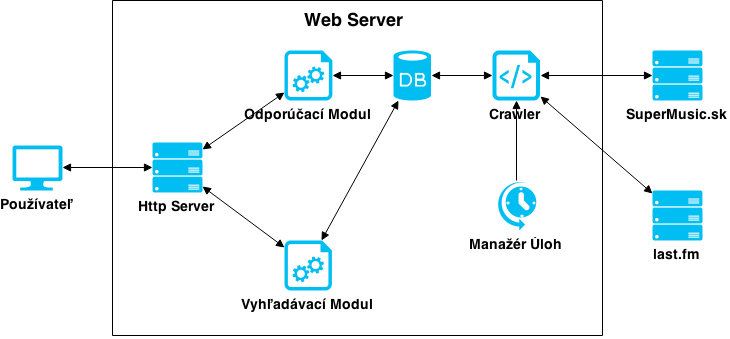
\includegraphics[scale=0.55]{app_structure}
        \caption{Štruktúra aplikácie}
        \label{fig:app_structure}
    \end{center}
\end{figure}

Aplikácia sa bude skladať z dôch hlavný oddelených subsystémov

\begin{itemize}
\item{odporúčanie (spúšťané používateľom cez prehliadač),}
\item{indexovanie dokumentov (séria úloh spúšťaná manažérom úloh).}
\end{itemize}

\subsection{Špecifikácia služieb}

Aplikácia by mala poskytovať niekoľko základných služieb

\begin{itemize}
\item{vyhľadávanie dokumentov,}
\item{najdenie podobných dokumentov aktuálne zobrazenému dokumentu,}
\item{odporúčanie dokumentov,}
\item{zostavenie spevníka.}
\end{itemize}

Prvé dve funkcionality sú vytvorené najmä z dôvodu že v danej doméne 
sa ťažko získavajú preferencie, ich jedinou úlohou je získanie základných
preferencií používateľa na základe ktorých budeme vytvárať odporúčania.

Pre zabezpečenie týchto funkcií bude potrebované udržiavať databázu dokumentov
ktorá sa bude pravidelne aktualizovať. Toto bude zabepečovať Kravler (angl. crawler)
ktorý bude vykonávať činnosti

\begin{itemize}
\item{prehľadávanie supermusic po nových dokuemntoch,}
\item{prehľadávanie supermusic po nových interprétoch,}
\item{sťahovanie dokumentov zo supermusic,}
\item{sťahovanie značiek z last.fm,}
\item{váhovanie značiek.}
\end{itemize}

Kravler bude implementovaný ako aplikácia pre príkazový riadok
aby sa dal použiť z manažérom úloh.

\paragraph{Odporúčanie}

Na odporúčanie by som chcel využiť filtrovanie na základe obsahu
spolú z vlastným algoritmom na určenie dlhodobých, krátkodobých a
sezonných záujmov.

\section{Implementácia}

\subsection{Datový model}

\paragraph{Model dokumentu}

Dokument bude reprezentovaný svojím názvom, typom a značkamy,
pričom zančky budú mať doménu na základe toho či vznikli
z názvu dokumentu, jeho typu, názvu interpréta alebo alebo
boli získane zo služby last.fm.

Čiže dokument bude uložený v trojrozmernom vektorovom priestore,
kde prvá súradnica budú dokumenty \(D = {d_1, d_2,... d_n}\),
ďaľšia súradnica budú značky \(Z = {z_1, z_2,.. z_n}\) a posledná 
súradnica budú domény \(D = {d_{názov}, d_{interpret}, d_{typ}, d_{tag}}\).

\paragraph{Model používateľa}

Používateľov profil bude reprezentovaný históriou navštívených značiek.
Bude sa ukladať pre každú navštívenu značku a jeden riadok bude obsahovať 
informácie \(row = {d_i, u_j, z_l, čas}\) kde \(d_i\) je zobrazený dokument,
\(u_j\) je používateľ ktorý dokument zobrazil, \(z_l\) je značka ktorá bola zobrazená.

Celú túto schému môžeme vydieť na obrázku \ref{fig:user_document_data_model}.


\begin{figure}
    \begin{center}
        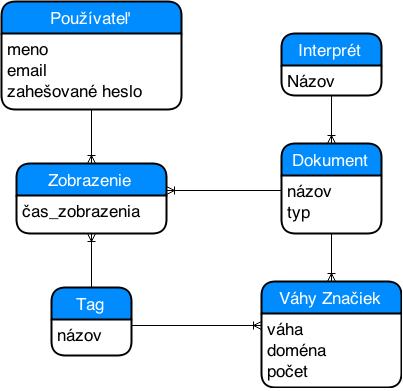
\includegraphics[scale=0.55]{user_document_data_model}
        \caption{Zjednodušený datový model}
        \label{fig:user_document_data_model}
    \end{center}
\end{figure}

\subsection{Indexovanie dokumentov a váhovanie}

\paragraph{Kravler}

Kravler (angl. crawler) je program slúžiacy na prehľadávanie webu za účelom
indexovania\footnote{http://en.wikipedia.org/wiki/Web\_crawler}. Kravler vykonáva niekoľko
operácií v rámci aplikácie, je implementovaný ako jednoduchý program príkazového riadku.
Každá z jeho operáci sa v prípade potreby dá vykonať osobytne. Toto je hlavne potrebné ak by
sa zmenili parametre indexovania. Na obrázku \ref{fig:crawler_flowchart} môžeme vydieť digram
akcií kravleru.

\begin{figure}
    \begin{center}
        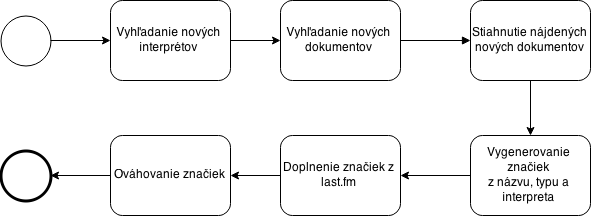
\includegraphics[scale=0.55]{crawler_flowchart}
        \caption{BPMN Digram kravleru}
        \label{fig:crawler_flowchart}
    \end{center}
\end{figure}

\paragraph{Vyhľadanie nových interpretov}

Táto akcia využíva spôsob akým sú na super music triedený interpreti.
Interpreti sa zobrazujú na stránke \uv{http://www.supermusic.sk/skupiny.php?od=}
pričom parameter \(od\) sú počiatošné písmena názvu kapely. Experimentálne 
som overil, že na prejdenie celej databázy potrebujem vygenerovať všetky trojpísmenové
začiatky názvou, pričom nezáleží na malích a veľkých písmenách. Pre generovaní používam 
anglickú abecedu až na prvé písmeno kde musím brať do úvahy aj niektorú diakritiku.

Prvé písmeno sa vyberá z množiny 
\uv{A, B, C, D, E, F, G, H, I, J, K, L, M, N, O, P, R, S, T, U, V, X, Y, *, Ž, Ť, Č}.
Tento príkaz sa dá spustiť aj paralélne, kedy vytvorí niekoľko 
 procesov, avšak príkaz nieje spoľahlivý, vzhľadom na to že v rámci zachovania portability 
som použil iba základnu knižnicu pcntl. Táto knižnica neobsahuje zámky, ani iný spôsob ako 
ošetriť prítupy ku zdrojom.

Kravler pre interpretov využíva XPath výrazy
[\ref{lst:interpret_id}, \ref{lst:interpret_name}, \ref{lst:interpret_alias}] na získanie 
dát zo stiahnutej stránky.

\begin{lstlisting}[caption=XPath na vyhľadanie interpretovho identifikátora,
    label=lst:interpret_id]
//table[@bgcolor="#333333" and position() = 2]//a/@id
\end{lstlisting}

\begin{lstlisting}[caption=XPath na vyhľadanie interpretovho mena,label=lst:interpret_name]
//table[@bgcolor="#333333" and position() = 2]//a/@href
\end{lstlisting}

\begin{lstlisting}[caption=XPath na vyhľadanie interpretovho aliasu,label=lst:interpret_alias]
//table[@bgcolor="#333333" and position() = 2]//a/text()
\end{lstlisting}

Tieto hodnoty sa ešte ďalej spracúvajú, napríklad vytiahnutie pri druhom XPath-te
\ref{lst:interpret_name} 
získame url z ktorej musíme aktuálne meno získať pomocou regulárneho výrazu.

\begin{lstlisting}[caption=Regulárny výraz na získanie mena interpreta z url interpreta,
    label=lst:regex_interpret_name]
/&name=.*\$/
\end{lstlisting}

\paragraph{Vyhľadanie nových dokumentov}

Táto akcia funguje podobne ako akcia akcia Vyhľadanie nových interpretov. Tiež genreuje adresy
z abecedy a adresy \uv{http://www.supermusic.sk/piesne.php?od=}.
pričom dopĺňa písmená na koniec adresy.

Prvý znak je anglická abeceda rozšírená o niekoľko slovenský a českých interpunkčný písmen
plus hviezda. Teda v provom rade sú písmená z množiny \uv{A, B, C, D, E, F, G, H, I, J, K, L, M,
N, O, P, Q, R, S, T, U, V, X, Y, Z, Č. Ď, Ľ, Ř, Š, Ť, Ž, *},
v druhej rade už je anglická abeceda.

Následne sa snaží získať zoznam piesni zo staihnutej stránky, za týmto účelom používam
XPath výrazy [\ref{lst:document_id}, \ref{lst:document_name}, \ref{lst:document_interpret}, 
\ref{lst:document_type}].

\begin{lstlisting}[caption=XPath na vyhľadanie názvou piesni,label=lst:document_name]
//table[@width=740]//td/a/text()
\end{lstlisting}

\begin{lstlisting}[caption=XPath na vyhľadanie názvou piesni,label=lst:document_id]
//table[@width=740]//td/a/@href
\end{lstlisting}

\begin{lstlisting}[caption=XPath na vyhľadanie názvou piesni,label=lst:document_type]
//table[@width=740]//td/imt/@src
\end{lstlisting}

\begin{lstlisting}[caption=XPath na vyhľadanie názvou piesni,label=lst:document_interpret]
//table[@width=740]//td/text()
\end{lstlisting}

\paragraph{Stiahnutie nových dokumentov}

Počas hľadania nových dokumentov sa ešte nesťahujú obsahy dokumentov. Takže 
všetky nové dokumenty ešte nemajú žiadný obsah, táto akcia si vyberie nové dokumenty
a následne ich sťahuj, url dokumenty sa dá získať tak že zoberiem url
\uv{http://www.supermusic.sk/skupina.php?action=piesen&idpiesne=} a na jej
koniec pridám identifikátor dokumentu.

Následne sa dokument spracuje, a ak to je potrebné prispôsobý sa aplikácií.

\paragraph{Vygenerovanie značiek}

Aby bolo možné odporúčať, je potrebné vygenerovať značky pre dokumenty. Značky
sa generujú z názvu dokument, názvu interpréta a typu dokumentu tak, že sa rozdelia na
slová. Následne sa odstrania slová zo slabou semantickou 
silou\footnote{http://en.wikipedia.org/wiki/Stop\_words}  (angl. stopwords).
Na filtrovanie takýchto slóv používa už hotový zoznam slóv vytvorený v rámci 
projektu stop-words\footnote{https://code.google.com/p/stop-words/}
Z tohoto projekty využívam sady

\begin{itemize}
\item{stop-words\_czech\_3\_cz,}
\item{stop-words\_english\_3\_en,}
\item{stop-words\_slovak\_2\_sk.}
\end{itemize}

Text sa ešte pre tým normalizuje a tak isto sa určí doména značky, pre jednoduchosť 
ukladania neukladám značku pre každú doménu osobytne, ale mám vytvorený číselník
ktorý priradzuje presné domény značkám. 

\begin{itemize}
\item{\(8\) znamená že značka je názov dokumentu aj názvo interpreta,}
\item{\(7\) znamená že značka je názov dokumentu a značka z názvu interpreta,}
\item{\(6\) znamená že značka je názov interpreta a značkou z názvu dokumentu,}
\item{\(5\) znamená že značka je názov dokumentu,}
\item{\(4\) znamená že značka je názov interpreta,}
\item{\(3\) znamená že značka je značkou v názve dokumentu aj interpreta,}
\item{\(2\) znamená že značka je značkou v názve dokumentu,}
\item{\(1\) znamená že značka je značkou v názve interpreta,}
\item{\(0\) znamená že značka je buď značka získana z typu dokumentu alebo služby last.fm.}
\end{itemize}

\paragraph{Doplnenie značiek z last.fm}

Na dopĺňanie značiek používam službu track.getTopTags z last.fm apy. Ktorá 
vráti pre interpreta a názvo piesne najčastejšie prideľované značky. Tie následne
pridám k danej piesni. Keďže počet pridelení vrátených z last.fm vysoko prebíjal
počty vytvorené z názvu dokumentu a interpreta, rozhodol som sa túto hodnotu 
nevyužiť.

\paragraph{Váhovanie značiek dokumentov}

Tento model sa v MySQL nazýva model prírodzeného jazyka (angl. Natural Language Model),
ktorý porovnáva vlastnosti dokumentov na základe abstrakcie priestoru,
v ktorom sú jednou dimenziou vlastnosti jedného dokuemntu a druhou vlastností druhého
dokumentu, prípade vyhľadávacieho reťazca alebo používateľský profil.
Následne sa vracajú dokumenty ktoré majú najpodobnejší smer vektora k požadovanej fráze.

V MySQL\footnote{http://dev.mysql.com/doc/internals/en/full-text-search.html}
je tento prístup implementovaný pomocov nasledujúcej 
rovnice \ref{eq:mysql_language_model}.

\begin{equation}\label{eq:mysql_language_model}
    w_d = \frac{\log(dtf_d) + 1}{\sum_{i=1}^{t} \log (dtf_i) + 1} .
        \frac{U}{1+0.0115 * U} .
        \log \frac {N}{nf}
\end{equation}

Rovnica obsahuje
\begin{itemize}
\item{\(dtf_d\) je množstvo koľko krát sa nachádza značka v dokumente,}
\item{\(dtf_i\) množstvo i-tej značky dokument,}
\item{\(U\) počet unikátnych značiek dokumentu, }
\item{\(N\) počet všetkých dokumentov, }
\item{\(nf\) je počet dokumentov ktoré obsahuje danú značku}
\end{itemize}

Rovnica sa dá rozdeliť na tri časti:

\begin{itemize}
\item{\textbf{Základná časť} je to primárna rovnica určujúca váhu pojmu,}
\item{\textbf{Normalizačný faktor} spôsobý, že ak je dokument kratší ako preiemerná dĺžka
dokuemntu, jeho relevancia stúpa. \cite{pivoted_doc_len}}
\item{\textbf{Inverzná frequencia} zabezpečuje že menej časté pojmy majú vyššiu váhu.}
\end{itemize}

\subsection{Odporúčanie}

V rámci odporúčania je vytvorených niekoľko algoritmov.

\paragraph{Agregované odporúčanie}

Ako referenčné odporúčanie som zvolil agregovanie všetkých zobrazených značiek, a vátenie
tých ktoré používateľ navštevoval najčastejšie. Matematicky je tento algoritmus vyjadrený
rovnicou \ref{eq:aggregated_recommendation},

\begin{equation}\label{eq:aggregated_recommendation}
u(d_i, u_k) = \sum\limit_{j = 0}^{j = N_{d_i u_k}} u(z_j)
\end{equation}

kde \(u(d_i, u_k)\) je užitočnosť dokumentu \(d_i\) pre používateľa \(u_k\),
ďalej \(N_{d_i u_k}\) čo je spoločný počet značiek dokumentu \(d_i\) a používateľa
\(u_k\) a \(u(z_j, d_i)\), čo je užitočnosť zančky \(z_j\) vzhľadom na dokument 
\(d_i\).

\paragraph{Vlastné odporúčanie}

Pri agregovanom odporúčaní však ale nastáva jeden zásadný problém, 
ak používateľ v istom čase zobrázy jeden dokument veľa krát, môže to tak ovplivniť 
jeho záujmi na dlhší čas. Napríklad na obrázku \ref{fig:casova_os} by značka 1 aj
značka 2 mala rovnakú váhu.

\begin{figure}
    \begin{center}
        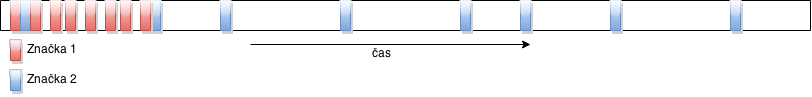
\includegraphics[scale=0.55]{casova_os}
        \caption{Zobrazenia značiek na časovej osy.}
        \label{fig:casova_os}
    \end{center}
\end{figure}

Na vyriešenie tohoto problému som sa rozhodol implementovať algoritmus, pri ktorom si 
rozdelím históriu zobrazení značiek na \(n\) rovnakých častí, značky v každej časti 
si zoradím podľa počtu zobrazení a vrátim si \(i\) najzobrazovanejších značiek. 
Pri každej časti považujem pozíciu na ktorej sa značka umiestnila za jej váhu.

Následne pre každú značku spočítam jej váhy zo všetkých skupín v ktorých sa vyskytla. 
Túto váhu nakoniec ešte zlogaritmuje z dôvodu že značky ktoré boli na prvých priečkach 
zvykli mať obrovský náskok oprotí nižším. Na ukážke \ref{lst:profile_tags} môžeme
vidieť pseudo kód tohoto algoritmu.

\begin{lstlisting}[label=lst:profile_tags, caption=Získanie značiek profilu]
Znacky ziskajZnackyProfilu(zobrazeneZnacky):
    znackyProfilu = []
    velkostJednejSkupiny = 
        pocet(zobrazeneZnacky) / configuracia('pocetSkupin')

    for i=0; i<pocet(zobrazeneZnacky); i+= velkostJednejSkupiny:
        zoskupeneZnacky = zoskup(
            zobrazeneZnacky, podla=znacky, pocet(*)
        )
        zoradeneZnacky = zorad(zoskupeneZnacky, podla=pocet(*))
        for j=0; j<configuracia('vrchSkupiny'); j++:
            znackyProfilu[zoradeneZnacky[j].nazov] += j;
    
    foreach znackyProfilu as znackaProfilu:
        znackaProfilu = log(znackaProfilu)
\end{lstlisting}

\paragraph{Skupinové odporúčanie}

Aplikácia tak isto umožňuje vytváranie spevníkov pre viacerích používateľov. Pre zjednodušenie
táto funkcionalita je implementovaná v dvoch krokoch. V prvom kroku sa získaju a ováhujú značky
vybranej skupiny používateľov, v druhom sa vrátia najužitočnejšie dokumenty na základe značiek.
Vyhodnotenie užitočnosti tagov zo zobrazení sa vypočítava podľa rovnice \ref{eq:group_recommend},

\begin{equation}\label{eq:group_recommend}
u(z_i) = \frac{N_{u_i}}{N_u} * \log (N_{z_i} + 1)
\end{equation}

kde \(u(z_i)\) je užitočnosť, \(N_{u_i}\) je počet používateľov ktorý už zobrazili značku
\(z_i\), \(N_u\) je počet používateľov pre ktorých chcem získať značky a \(\N_{z_i}\) je 
celkový počet zobrazení značky.

\paragraph{Podobnosť dokumentov}

Pre vylepšenie odporúčanií počas prieskumného vyhľadávania, beriem do úvahy aj dokument ktorý
sa najviac podobá na aktuálny dokument. Podobnosť dokumentov je vyhodnotená pomocov rovnice
\ref{eq:doc_similiarity}.

\begin{equation}\label{eq:doc_similiarity}
podobnost(d_i, d_j) = \sum\limit_{k = 0}^{N_{ij}} u(d_i, z_k) * u(d_j, z_k)
\end{equation}

kde \(N_{ij}\) je počet spoločných značiek dokumentu \(d_i\) a dokumentu \(d_j\) a 
\(d_i, z_k\) je užitočnosť značky \(z_k\) vzhľadom na dokument \(d_i\).

\paragraph{Porovnávanie z dokumentom}

Dokument môžem porovnať z akou koľvek sadou ováhovaných značiek, či už vytvorenej z profilu 
používateľa alebo z vyhľadávacieho reťazca. Toto porovnávanie je vyjadrené rovnicou
\ref{eq:document_match}.

\begin{equation}\label{eq:document_match}
vyhovuje(d_i, Z) = \sum\limit_{k = 0}^{N_{z}} u(d_i, z_k) * qu(z_k)
\end{equation}

kde \(Z\) je sada značiek pre ktorú sa snažím najsť vyhovujúci dokument. \(N_z\) je počet značiek
ktoré má dokument a sada značiek na porovnanie rovnaké, \(u(d_i, z_k)\) je užitočnosť značky
\(k\) vzhľadom na dokument \(d_i\) a \(qu(z_k)\) je užitočnosť značky \(z_k\) v sade značiek
\(Z\).

%\paragraph{Priama tagovacia tabuľka}
%
%Vytvoril som tabuľku tagov, kde bol každý tag fyzický priamo vložený spolu z id dokumentu ku ktoremu sa viaže,
%tento prístup ale nebol dostatočne rýchli na vygenerovanie, ani na vyhľadávanie. Pri vyhľadávaní nad 118989 značkamy 
%označujúcimi 47002 dokumentov zabral 44.6984 sekúnd. Nepomohlo ani zindexovanie podľa mena.
%
%\subsection{Váhovanie Dokumentu}
%
%\[w(d_j) = \sum_{i=1}^{N} w(t_i) \]
%
%\begin{itemize}
%\item{\(N\)} Počet značiek v dokumente,
%\item{\(t_i\)} I-ty pojem v dokumente,
%\item{\(d_j\)} J-ty dokument.
%\end{itemize}

%\section{Návrh, špecifikácia požiadaviek a pod.}
%Aenean consequat, sapien a posuere tincidunt, massa purus egestas nisl, sed sollicitudin neque mi vel augue. Sed condimentum nibh ut metus condimentum ornare. Maecenas ultrices tempor condimentum. Etiam nec lorem leo, id consequat tellus. Etiam id mattis massa. Phasellus commodo, lacus in viverra lacinia, quam leo ultricies tellus, condimentum vehicula dui nisl a magna. In mi felis, malesuada eget tincidunt eget, rutrum ac lacus. In a nisl tellus. Mauris hendrerit egestas odio ac consequat. Curabitur aliquam convallis nibh sed blandit. Ut et viverra felis. Sed varius quam non mauris facilisis tincidunt. Quisque et libero eros, sed hendrerit sapien. Aliquam nec faucibus neque. Integer dictum arcu sed risus scelerisque fermentum. Pellentesque vitae ipsum lorem, sed lacinia ligula~\cite{4}.
%
%\begin{figure}\begin{center}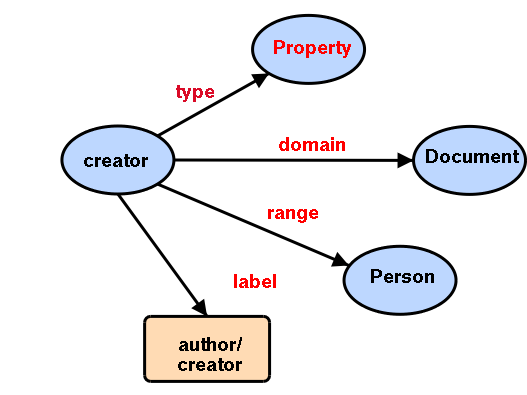
\includegraphics[scale=0.55]{figure2}
%\caption{Popis schémy.}\label{figure2}
%\end{center}\end{figure}
%
%Etiam nec lorem leo, id consequat tellus. Etiam id mattis massa. Phasellus commodo, lacus in viverra lacinia, quam leo ultricies tellus, condimentum vehicula dui nisl a magna. In mi felis, malesuada eget tincidunt eget, rutrum ac lacus. In a nisl tellus. Mauris hendrerit egestas odio ac consequat. Etiam nec lorem leo, id consequat tellus. Etiam id mattis massa. Phasellus commodo, lacus in viverra lacinia, quam leo ultricies tellus, condimentum vehicula dui nisl a magna. In mi felis, malesuada eget tincidunt eget, rutrum ac lacus. In a nisl tellus. Mauris hendrerit egestas odio ac consequat. Etiam nec lorem leo, id consequat tellus. Etiam id mattis massa. Phasellus commodo, lacus in viverra lacinia, quam leo ultricies tellus, condimentum vehicula dui nisl a magna. In mi felis, malesuada eget tincidunt eget, rutrum ac lacus. In a nisl tellus. Mauris hendrerit egestas odio ac consequat.
%
%\lstinputlisting[float=h,language=javascript,caption={Príklad listingu zo súboru.},label={listing},frame=single,frameround=ffff,captionpos=b,basicstyle=\scriptsize]{figures/listing}
%
%Etiam nec lorem leo, id consequat tellus. Etiam id mattis massa. Phasellus commodo, lacus in viverra lacinia, quam leo ultricies tellus, condimentum vehicula dui nisl a magna. In mi felis, malesuada eget tincidunt eget, rutrum ac lacus. In a nisl tellus. Mauris hendrerit egestas odio ac consequat. Etiam nec lorem leo, id consequat tellus. Etiam id mattis massa. Phasellus commodo, lacus in viverra lacinia, quam leo ultricies tellus, condimentum vehicula dui nisl a magna. In mi felis, malesuada eget tincidunt eget, rutrum ac lacus. In a nisl tellus. Mauris hendrerit egestas odio ac consequat. Etiam nec lorem leo, id consequat tellus. Etiam id mattis massa. Phasellus commodo, lacus in viverra lacinia, quam leo ultricies tellus, condimentum vehicula dui nisl a magna. In mi felis, malesuada eget tincidunt eget, rutrum ac lacus. In a nisl tellus. Mauris hendrerit egestas odio ac consequat.

